\documentclass[aspectratio=43]{beamer}
\usepackage[latin1]{inputenc}
\usepackage{amsmath}
\usepackage{amsfonts}
\usepackage{amssymb}
\usepackage{makeidx}
\usepackage{graphicx}
\usepackage{array}

% Customization
\mode<presentation>{
\usetheme{CambridgeUS}
\usecolortheme{dolphin}
\setbeamertemplate{navigation symbols}{}
}

%\setbeamertemplate{footline}[frame number]

%TikZ diagrams
\usepackage{tikz}
\usetikzlibrary{patterns}
\usetikzlibrary{arrows,shapes}
\usetikzlibrary{shapes.multipart}
\usetikzlibrary{trees}
\usetikzlibrary{shapes.geometric}
\usetikzlibrary{matrix,arrows}
\usetikzlibrary{positioning}
\usetikzlibrary{calc,through}
\usetikzlibrary{decorations.pathreplacing}
\usepackage{pgffor}

% Define colors
\definecolor{darkgreen}{rgb}{0.0, 0.5, 0.13}
\definecolor{darkblue}{rgb}{0.0, 0.0, 0.55}
\definecolor{darkred}{rgb}{0.55, 0.0, 0.0}

% For using TikZ
\usetikzlibrary{decorations.pathmorphing}
\usetikzlibrary{decorations.markings}
\tikzset{
	vector/.style={decorate, decoration={snake,amplitude=3pt}, draw},
	gluon/.style={decorate, decoration={coil,amplitude=2.5pt},draw},
	provector/.style={decorate, decoration={snake,amplitude=2.5pt}, draw},
	antivector/.style={decorate, decoration={snake,amplitude=-2.5pt}, draw},
	fermion/.style={draw=black, postaction={decorate},
		decoration={markings,mark=at position .55 with {\arrow[draw=black,thick]{>}}}},
	fermionbar/.style={draw=black, postaction={decorate},
		decoration={markings,mark=at position .55 with {\arrow[draw=black,thick]{<}}}},
	fermionnoarrow/.style={draw=black},
	gluon/.style={decorate, draw=black,
		decoration={coil,amplitude=2.5pt, segment length=3pt}},
	gluon2/.style={decorate, draw=black,
		decoration={coil,amplitude=1.75pt, segment length=2.75pt}},
	scalar/.style={dashed,draw=black, postaction={decorate},
		decoration={markings,mark=at position .55 with {\arrow[draw=black]{>}}}},
	scalarbar/.style={dashed,draw=black, postaction={decorate},
		decoration={markings,mark=at position .55 with {\arrow[draw=black]{<}}}},
	scalarnoarrow/.style={dashed,draw=black},
	electron/.style={draw=black, postaction={decorate},
		decoration={markings,mark=at position .55 with {\arrow[draw=black]{>}}}},
	bigvector/.style={decorate, decoration={snake,amplitude=4pt}, draw},
}

% Blocks
\tikzstyle{block} = [draw, rectangle, minimum height = 3em, rounded corners, minimum width = 4em]
\tikzstyle{block2} = [draw, rectangle, minimum height = 3em, rounded corners, minimum width = 7em]
\tikzstyle{circle} = [draw, circle, radius = 1.5]
\tikzstyle{arrow} = [thick,->]
%************************************************************************************************************

% Title and author
\title[QCD predictions for Higgs production]{QCD predictions for Higgs production}
\author{\textbf {Jes\'us Urtasun Elizari}}
%\institute{\textbf {University of Milan}}
\date{Milan, September 2020}

\begin{document}

% Front slide
\begin{frame}

	%\maketitle
	\vspace{1.0 cm}
	
	\center{\color{blue}High precision perturbative QCD predictions \\ for Higgs production at the LHC}
	
	\vspace{0.25 cm}
	\center{Jes\'us Urtasun Elizari}
	\center{PhD seminar - Milan, September 2020}

	\begin{figure}
		\minipage{1\textwidth}
		
\includegraphics[width = 3.0 cm]{plots/unimi.png}
		\hfill
		
\includegraphics[width = 3.0 cm]{plots/n3pdf.png}
		\hfill
		
\includegraphics[width = 3.0 cm]{plots/erc.png}
		\endminipage
	\end{figure}

	\vspace{1.0 cm}
	
	{\scriptsize \color{blue} This project has received funding from the European Union$'$s Horizon 2020 research and innovation program under grant agreement No 740006.}

\end{frame}

% Introduction
\begin{frame}

	\frametitle{Outline}
	
	\begin{enumerate}
		\item {\color{blue}QCD in a nutshell}
		\begin{itemize}
			\item Factorization in QCD
			\item Partonic cross section
			\item Perturbative QCD
		\end{itemize}
		\item {\color{blue}Resummation in QCD}
		\begin{itemize}
			\item Higher order corrections
			\item Resummation of $q_{\perp}$
		\end{itemize}
		\item {\color{blue}HTurbo}
		\begin{itemize}
			\item Higgs production at the LHC: HRes and HqT
			\item HTurbo: Fast predictions for Higgs production
			\item Results $\&$ Conclusions
		\end{itemize}
	\end{enumerate}
	
\end{frame}

% QCD in a nutshell
\begin{frame}

	\center{\color{blue}QCD in a nutshell}

\end{frame}

% LHC physics
\begin{frame}

	\frametitle{QCD in a nutshell}
	\framesubtitle{LHC physics}
	
	\begin{figure}
		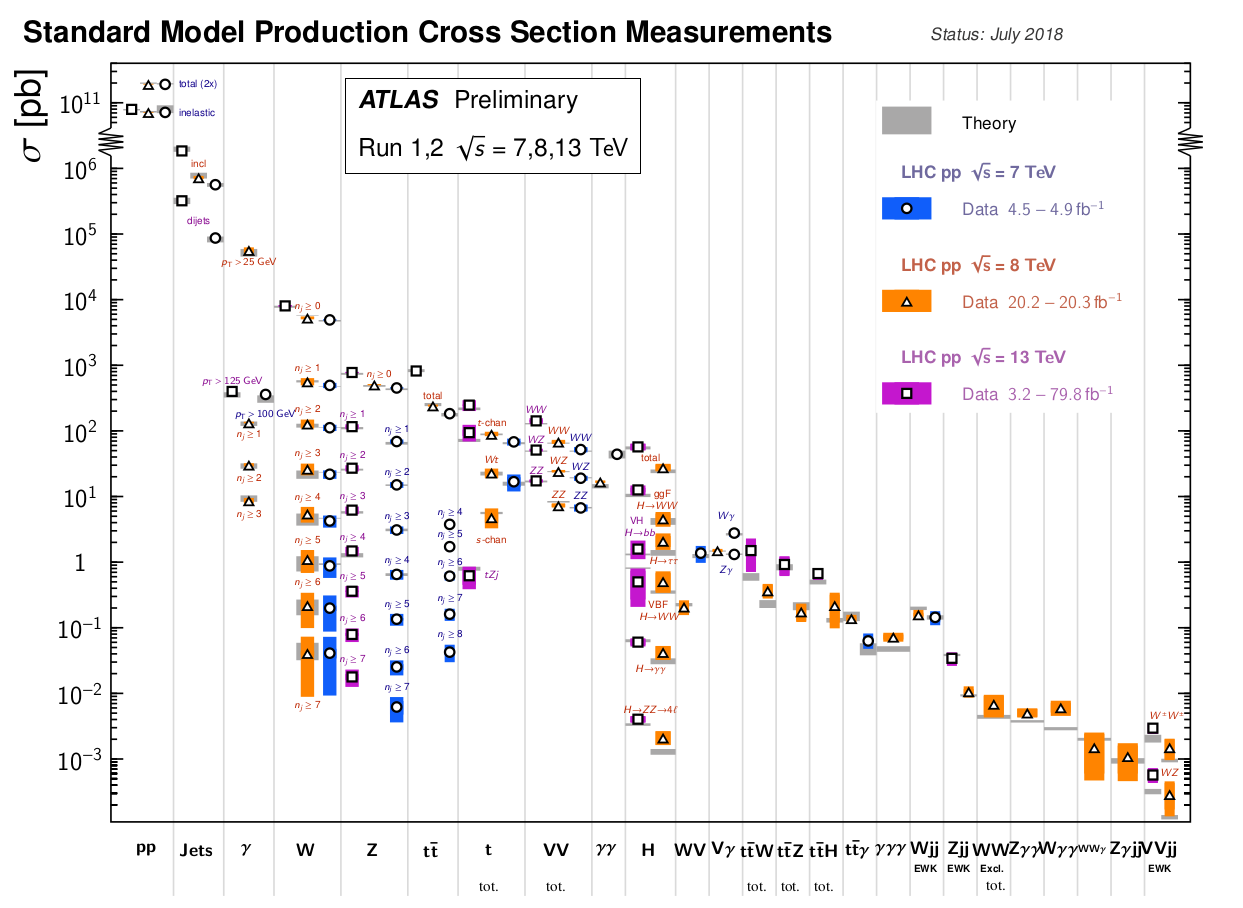
\includegraphics[width = 9.5 cm]{plots/lhc_measurements.png}
	\end{figure}

\end{frame}

% Factorization theorem
\begin{frame}

	\frametitle{QCD in a nutshell}
	\framesubtitle{Factorization theorem}

	\begin{figure}
		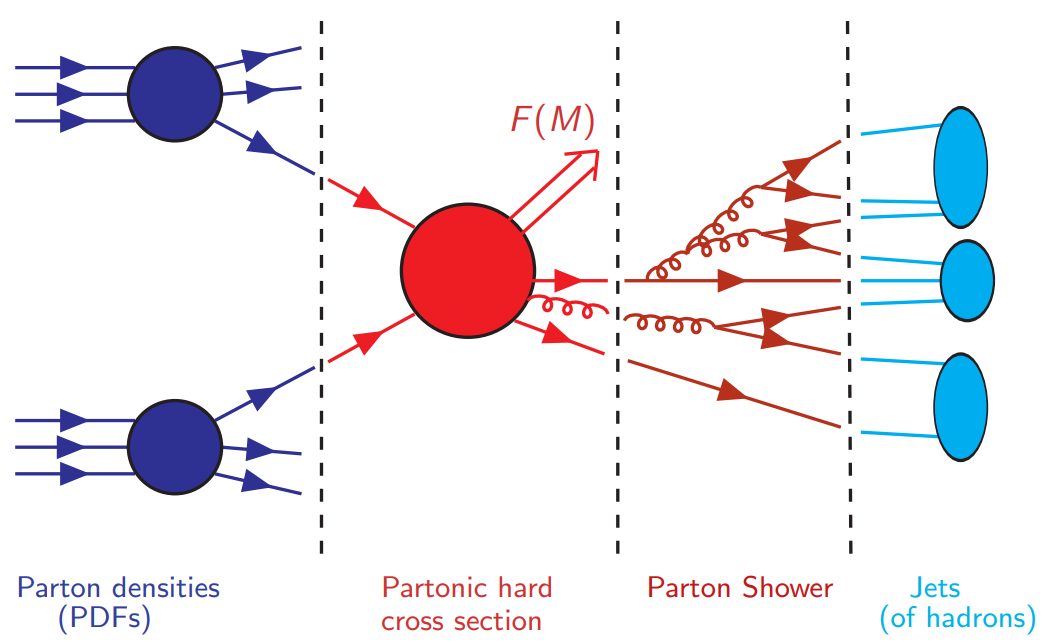
\includegraphics[width = 7 cm]{plots/factorization_1.png}
	\end{figure}
	
	Compute cross sections is a {\color{red}Hard problem} $\longrightarrow$ {\color{blue} QCD Factorization}
	
	\begin{equation}
		\sigma^{\textrm{F}}(p_{1}, p_{2}) =
		\int_{0}^{1} dx_{1} dx_{2} \; {\color{blue} f_{\alpha}(x_{1}, \mu_{F}^{2}) \ast f_{\beta}(x_{2}, \mu_{F}^{2})}
		\; \ast \;  
		{\color{red}\hat{\sigma}^{\textrm{F}}_{\alpha \beta}(x_{1}p_{1}, x_{2}p_{2}, \alpha_{s}(\mu_{R}^{2}), \mu_{F}^{2})} \nonumber
	\end{equation}

\end{frame}

% Partonic cross section
\begin{frame}
	
	\frametitle{QCD in a nutshell}
	\framesubtitle{Partonic cross section}
	
	\begin{figure}
		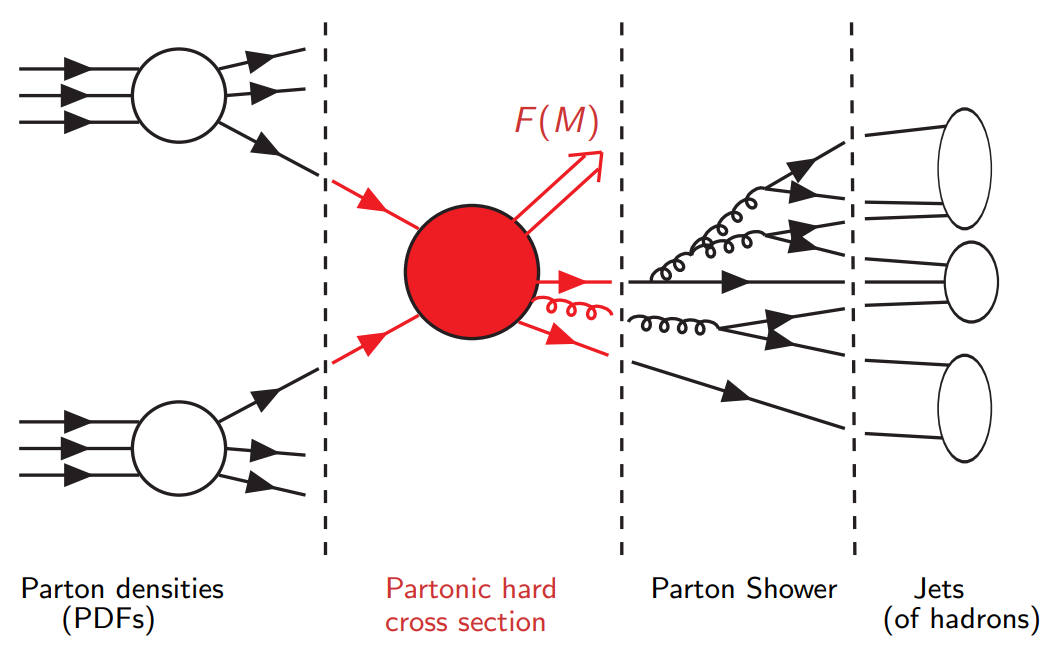
\includegraphics[width = 7 cm]{plots/factorization_2.png}
	\end{figure}
	
	\begin{itemize}
		\item {\color{blue}PDFs} ${\color{blue} f_{\alpha}(x_{i}, \mu_{F}^{2})}$ absorb the non perturbative effects, evaluated at $\mu_{F}$
		\item Partonic {\color{red}$\hat{\sigma}^{\textrm{F}}_{\alpha \beta}$} can be computed as perturbative series in $\alpha_{s}$
	\end{itemize}
	
\end{frame}

% Perturbative QCD
\begin{frame}

	\frametitle{QCD in a nutshell}
	\framesubtitle{Perturbative QCD}
	
	\begin{columns}
		
		\column{0.45\textwidth}
		
		\begin{itemize}
			\item Born cross section as LO value of a perturbative series
			\item $\sigma^{(1)}, \sigma^{(2)}, \sigma^{(3)}$ are the NLO, NNLO, N3LO corrections
		\end{itemize}
		
		\column{0.45\textwidth}
		\begin{figure}[!htb]
			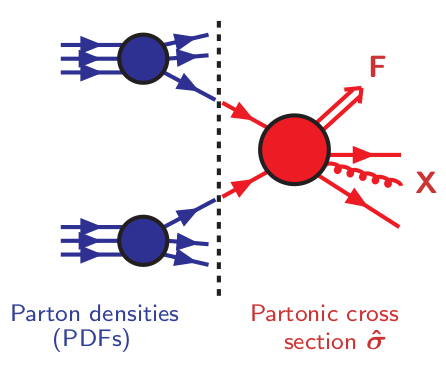
\includegraphics[width = 5 cm]{plots/factorization_3.png}
		\end{figure}
	
	\end{columns}
	
	\begin{equation}
		\hat{\sigma} = \sigma^{\texttt{Born}} \Bigg( 1 +
		\frac{\alpha_{s}}{2\pi} \sigma^{(1)} + 
		\Big(\frac{\alpha_{s}}{2\pi}\Big)^{2} \sigma^{(2)} + 
		\Big(\frac{\alpha_{s}}{2\pi}\Big)^{3} \sigma^{(3)} + ... \Bigg) \nonumber
	\end{equation}
	
	Leading order predictions can strongly depend on the renormalization and factorization scales $\rightarrow$ {\color{red}Need higher order corrections!}

\end{frame}

% Dealing with divergences
\begin{frame}

	\center{\color{blue}Resummation in QCD}

\end{frame}

% Higher order corrections
\begin{frame}

	\frametitle{Resummation in QCD}
	\framesubtitle{Higher order corrections}
	\begin{columns}
	
	\column{0.45\textwidth}
	
	\begin{enumerate}
		\item Higher order corrections are {\color{red}not an easy task} due to {\color{red} infrared (IR) singularities}
		\item Final state radiations cancel by combining real and virtual contributions
		\item Initial state radiations factorized inside the PDFs, then {\color{blue} IR-free, finite $\hat{\sigma}$}
	\end{enumerate}
	
	\column{0.45\textwidth}
	\begin{figure}[!htb]
		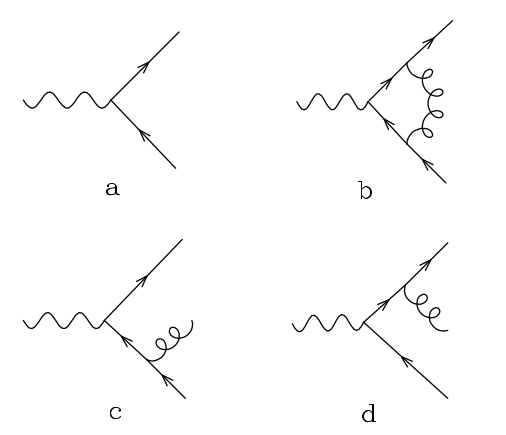
\includegraphics[width = \linewidth]{plots/qcd_corrections.png}
	\end{figure}
	
	\end{columns}

\end{frame}

% qT resummation I
\begin{frame}

	\frametitle{Resummation in QCD}
	\framesubtitle{$q_{\perp}$ resummation}
	
	\center	Study the differential $q_{\perp}$ distribution \\
	\center	$h_{1}(p_{1}) + h_{2}(p_{2}) \longrightarrow F(M, {\color{red}q_{\perp}}) + X$
	
	\begin{columns}
	
	\column{0.55\textwidth}

	\begin{figure}
		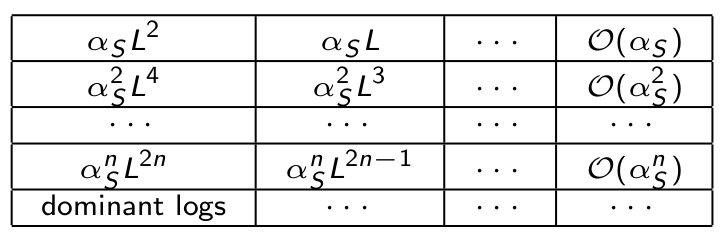
\includegraphics[width = 7.5cm]{plots/qT_logs_table.png}
	\end{figure}

	\column{0.45\textwidth}
	
	\begin{figure}
		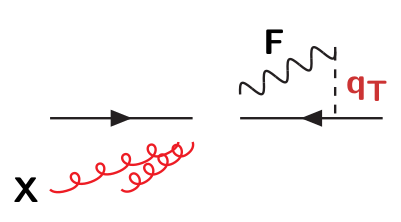
\includegraphics[width = 4cm]{plots/qT_diagram.png}
	\end{figure}

	\end{columns}

	\vspace{0.5 cm}

	Truncated fixed order predictions $\rightarrow$ {\color{red}divergent $\alpha_{s}^{n}\ln^{m}(M^{2}/q_{\perp}^{2})$ appear}

\end{frame}

% Resummation in QCD II
\begin{frame}

	\frametitle{Resummation in QCD}
	\framesubtitle{$q_{\perp}$ resummation}

	Replace partonic $q_{\perp}$ distribution as follows
	
	\begin{equation}
		\frac{d\hat{\sigma}_{ab}}{dq_{\perp}^{2}} \rightarrow 
		\Bigg[ \frac{d\hat{\sigma}^{\textrm{(res.)}}_{ab}}{dq_{\perp}^{2}} \Bigg]_{\textrm{l.a.}} + 
		\Bigg[ \frac{d\hat{\sigma}^{\textrm{(fin.)}}_{ab}}{dq_{\perp}^{2}} \Bigg]_{\textrm{f.o.}} \textrm{\quad, such that} \nonumber
	\end{equation}

	\begin{align}
		\int dq_{\perp}^{2} \frac{d\hat{\sigma}^{\textrm{(res.)}}_{ab}}{dq_{\perp}^{2}} &\sim \sum \alpha_{s}^{n} \log^{m} \frac{M^{2}}{Q_{\perp}^{2}} \textrm{\quad for \quad} q_{\perp} \rightarrow 0 \nonumber \\
		\int dq_{\perp}^{2} \frac{d\hat{\sigma}^{\textrm{(fin.)}}_{ab}}{dq_{\perp}^{2}} &\sim 0 \nonumber \textrm{\quad for \quad} q_{\perp} \rightarrow 0
	\end{align}

	Resummed and finite components need to be matched at some logarithmic accuracy (LL, NLL, NNLL, ...)

\end{frame}

% qT resummation III
\begin{frame}

	\frametitle{Resummation in QCD}
	\framesubtitle{$q_{\perp}$ resummation}
	
	Resummation holds in impact parameter space $b$
	\begin{equation}
		\frac{d\hat{\sigma}_{ab}^{\textrm{(res.)}}}{dq_{\perp}^{2}} = \frac{M^{2}}{\hat{s}} \int db \; \frac{b}{2} \; J_{0}(b q_{\perp}) \; {\color{red} \mathcal{W}_{ab}(b, M)} \nonumber
	\end{equation}
	
	Which is expressed in Mellin space (with respect to $z = M^{2}/\hat{s}$)
	\begin{equation}
		{\color{red} \mathcal{W}_{N}(b, M) = \mathcal{H}_{N}(\alpha_{s}) \times \exp\{\mathcal{G}_{N}(\alpha_{s}, L)\}} \quad\textrm{being}\quad L \equiv \log(M^{2}b^{2}) \nonumber
	\end{equation}

	\begin{itemize}
		\item Resummed effects exponentiated in the Sudakov factor {\color{red}$\mathcal{G}_{N}(\alpha_{s}, L)$}
		\item Process-dependence factorized in the hard factor {\color{red}$\mathcal{H}_{N}(\alpha_{s})$}
	\end{itemize}

	
\end{frame}

% HTurbo
\begin{frame}

	\center{\color{blue}HTurbo: Fast predictions for Higgs production}

\end{frame}

% HqT and HRes
\begin{frame}

	\frametitle{HqT and HRes}
	\framesubtitle{Predictions for Higgs $q_{\perp}$ distribution}
	
	\begin{columns}
		
		\column{0.45\textwidth}
			
		\begin{itemize}
			\item HqT and HRes {\color{blue}[de Florian, G.F., Grazzini, Tommasini]} produce $q_{\perp}$ distributions
			\item Higher order corrections require {\color{red}high computation times}
			\item Codes producing fast predictions are needed for precision era of the LHC
		\end{itemize}

		\column{0.55\textwidth}
	
		\begin{figure}
			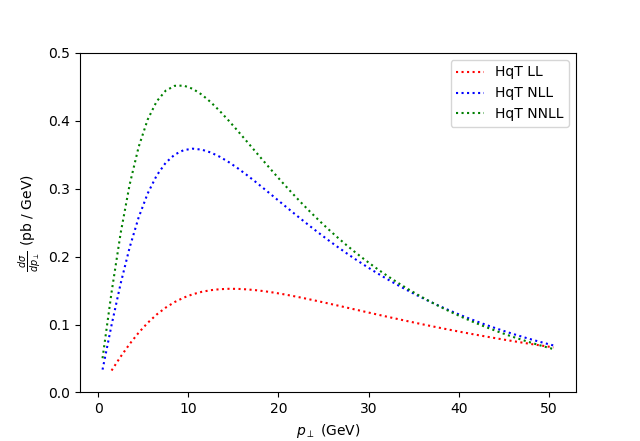
\includegraphics[width = 7 cm]{plots/higgs_qt_all.png}
		\end{figure}		
			
	\end{columns}

\end{frame}

% DYturbo I
\begin{frame}

	\frametitle{HTurbo}
	\framesubtitle{Starting point DYTurbo}
		
	\begin{itemize}
		\item Start from \textbf{DYTurbo} [Camarda et al.] ref. at {\color{blue} \href{https://arxiv.org/abs/1910.07049}{1910.07049}}, producing $q_{\perp}$ distribution fro Drell-Yan ($q\bar{q} \rightarrow l^{+}l^{-}$) 
	\end{itemize}
	
	{\color{blue}C++} interface rather that {\color{red}Fortran} of \textbf{HRes} or \textbf{HqT}
	
	\begin{itemize}
		\item Set LO amplitude $gg \rightarrow H$
		\item Set Sudakov and Hard coefficients for Higgs production
		\item Implement PDF evolution
		\item Compare with \textbf{HRes} and \textbf{HqT}
	\end{itemize}

	\vspace{0.5 cm}

	{\color{red} State of the art is just up to NNLL!}

\end{frame}

% DYturbo II
\begin{frame}

	\frametitle{HTurbo}
	\framesubtitle{Starting point DYTurbo}
	
	\begin{itemize}
		\item Set LO amplitude to be $gg \rightarrow H$
		\item Set Sudakov and Hard coefficients for Higgs production
		\item Compare with \textbf{HRes} and \textbf{HqT}
	\end{itemize}
	
	\begin{align}
		\mathcal{G}_{N}(\alpha_{s}, L) &= L\;g^{(1)}(\alpha_{s}L) + g^{(2)}(\alpha_{s}L) + \frac{\alpha_{s}}{\pi}g^{(3)}(\alpha_{s}L) + ... \nonumber \\
		\mathcal{H}_{N}(\alpha_{s}) &= 1 + \frac{\alpha_{s}}{\pi}\mathcal{H}^{(1)} + \Big(\frac{\alpha_{s}}{\pi}\Big)^{2}\mathcal{H}^{(2)} + ...  \nonumber
	\end{align}
	
	\begin{columns}
		
		\column{0.45\textwidth}

		\begin{align}
			&\textrm{LL} (\sim \alpha_{s}^{n}L^{n+1}): g^{(1)}, \hat{\sigma}^{(0)} \nonumber \\
			&\textrm{NLL} (\sim \alpha_{s}^{n}L^{n}): g^{(2)}, \mathcal{H}^{(1)} \nonumber \\
			&\textrm{NNLL} (\sim \alpha_{s}^{n}L^{n-1}): g^{(3)}, \mathcal{H}^{(2)} \nonumber
		\end{align}
	
		\column{0.45\textwidth}
		
		Start by building predictions up to NNLO, then add {\color{blue}N$^{3}$LL}
		
	\end{columns}

\end{frame}

% Results LL
\begin{frame}
	
	\frametitle{Results}
	\framesubtitle{Comparison HTurbo and HqT - LL}
	
	\begin{figure}
		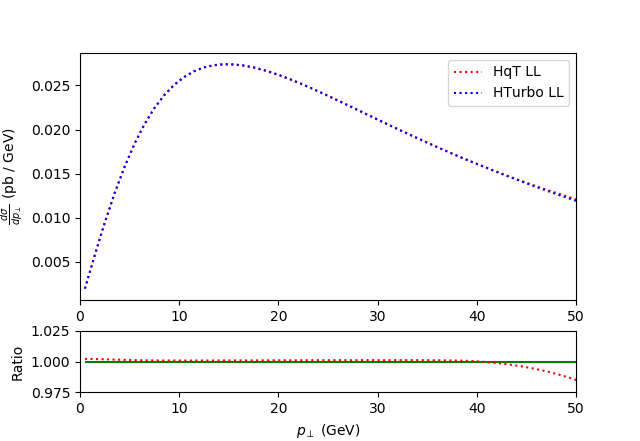
\includegraphics[width = 8cm]{plots/hturbo_LL.png}
	\end{figure}
	
	\begin{itemize}
		\item HTurbo $q_{\perp}$ distribution matches HRes and HqT at LL
		\item Excellent numerical agreement up to the 1/1000 level
	\end{itemize}

\end{frame}

% Results NLL
\begin{frame}

	\frametitle{Results}
	\framesubtitle{Comparison HTurbo and HqT - NLL}
	
	\begin{figure}
		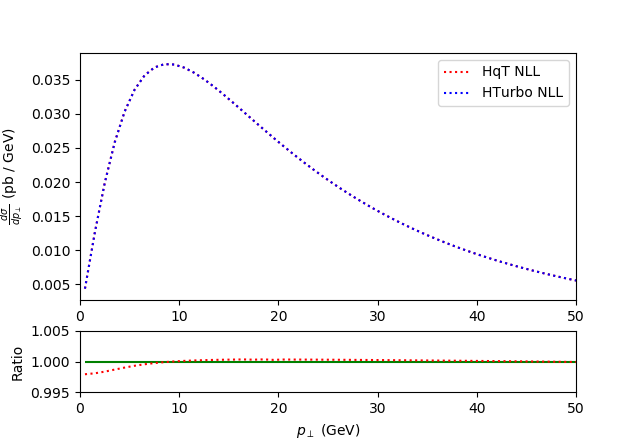
\includegraphics[width = 8cm]{plots/hturbo_NLL_noevol.png}
	\end{figure}
	
	\begin{itemize}
		\item HTurbo $q_{\perp}$ distribution matches HRes and HqT at NLL
		\item Agreement obtained by switching off PDF evolution
	\end{itemize}

\end{frame}

% Results NNLL
\begin{frame}

	\frametitle{Results}
	\framesubtitle{Comparison HTurbo and HqT - NNLL}
	
	\begin{figure}
		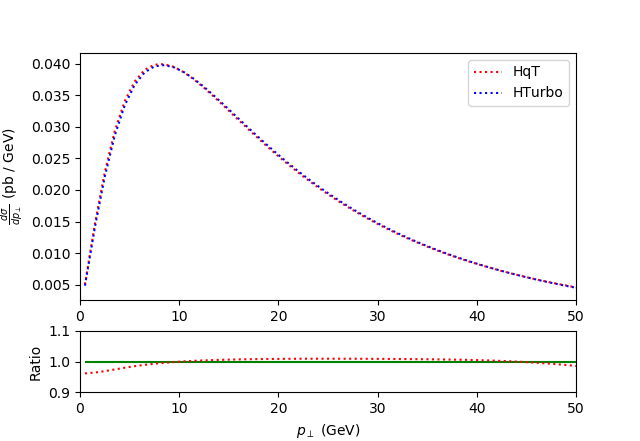
\includegraphics[width = 8cm]{plots/hturbo_NNLL_f2only2.png}
	\end{figure}
	
	\begin{itemize}
		\item HTurbo $q_{\perp}$ distribution matches HRes and HqT at NNLL
		\item Agreement obtained by switching off PDF evolution
\end{itemize}

\end{frame}

% Results all
\begin{frame}
	
	\frametitle{Results}
	\framesubtitle{Comparison HTurbo and HqT - all orders}
	
	\begin{figure}
		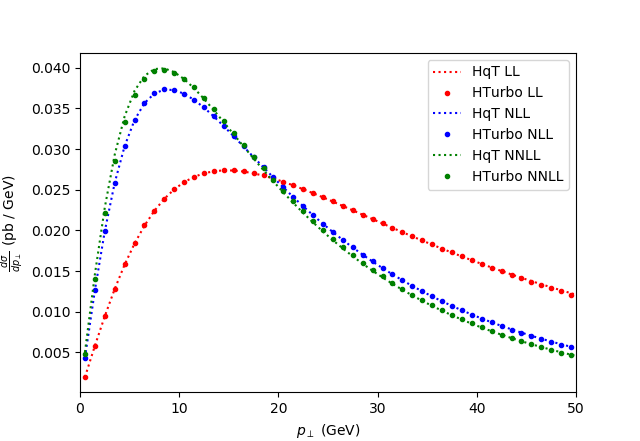
\includegraphics[width = 8cm]{plots/hturbo_all_noevol.png}
	\end{figure}
	
	\begin{itemize}
		\item Higher orders lead to more reliable predictions {\color{darkgreen}$\checkmark$} 
		\item Agreement up to NNLL $\longrightarrow$ {\color{blue}ready for N$^{3}$LL}
	\end{itemize}

\end{frame}

% Conclusions
\begin{frame}
	
	\frametitle{Summary $\&$ Conclusions}

	\vspace{2.0 cm}
	
	\begin{enumerate}
		\item Fast predictions are required towards the precision era of the LHC
		\item $q_{\perp}$ distributions from HTurbo {\color{blue}match HRes and HqT up to NNLL}
		\item HTurbo is {\color{blue}much faster than any of the existing Higgs codes}
		\item Next steps: Implement PDF evolution and {\color{blue}N$^{3}$LO distributions}

	\end{enumerate}

	\vspace{2.0 cm}

\end{frame}

% Conclusions
\begin{frame}

	\center {\color{blue}Thank you!}

	\begin{figure}
		
\includegraphics[width = 4 cm]{plots/thinking.png}
	\end{figure}		

	{\small \color{blue} This project has received funding from the European Union$'$s Horizon 2020 research and innovation program under grant agreement No 740006.}

\end{frame}


\end{document}